% Style for a MSc paper at Warsaw School of Economics
% Michał Ramsza
% xD
% Friday, December 14, 2012

% --- document class and other global stuff ---------------------------
\documentclass[polish, twoside, 12pt, a4paper]{article}

% --- packages --------------------------------------------------------
\usepackage{textcomp}
\usepackage{times}
\usepackage{amsmath}
\usepackage{amsfonts}
\usepackage{amssymb}
\usepackage{amsthm}
\usepackage[T1]{fontenc}
\usepackage[utf8]{inputenc}
\usepackage{graphicx}
\usepackage{xcolor}
\usepackage{enumitem}
\usepackage[polish]{babel}
\usepackage[centering, left=3.5cm, right=2.5cm, textheight=24cm]{geometry}

% --- packages for citations ------------------------------------------
\usepackage{natbib}
\AtBeginDocument{\renewcommand{\harvardand}{i}}

% --- package for automatic insertion of R code -----------------------
\usepackage{listings}
\lstset{language=R,%
   numbers=left,%
   tabsize=3,%
   numberstyle=\footnotesize,%
   basicstyle=\ttfamily \footnotesize \color{black},%
   escapeinside={(*@}{@*)}}

% --- support for links -----------------------------------------------	
\usepackage{url}
\usepackage{hyperref}
\hypersetup{colorlinks=true,
            linkcolor=black,
            citecolor=darkgray,
            urlcolor=darkgray,
            pagecolor=darkgray}

% --- support for large tables and other stuff ------------------------	
\usepackage{longtable}
%\usepackage{subfigure} % this package will now work with subcaption package
\usepackage{float}
\usepackage{caption}
\usepackage{subcaption}


% --- definitions for environments -------------------------------------
\theoremstyle{definition}
    \newtheorem{condition}{Assumption}
    \newtheorem{example}{Example}      

\theoremstyle{plain}
    \newtheorem{definition}{Definition}    
    \newtheorem{proposition}{Proposition}
    \newtheorem{theorem}{Theorem}
    \newtheorem{cor}{Corollary}

\theoremstyle{remark}
    \newtheorem{remark}{Remark}

% --- other settings --------------------------------------------------
\linespread{1.5}
\frenchspacing
\sloppy
\allowdisplaybreaks[4]
\raggedbottom
\clubpenalty=10000
\widowpenalty=10000

% --- only if required ------------------------------------------------
\AtBeginDocument{\renewcommand*{\figurename}{Wykres}}
\AtBeginDocument{\renewcommand*{\tablename}{Tabela}}

% ---------------------------------------------------------------------
\begin{document}

% --- strona tytulowa -------------------------------------------------
\begin{titlepage}
\centering


\includegraphics[scale=0.6]{uw_logo.JPG}
\\[20pt]


\vspace*{0.5cm}
Studium magisterskie\\
\begin{flushleft}
Kierunek: Informatyka i Ekonometria\\
Forma studiów: stacjonarne
\end{flushleft}

\vspace*{.5cm}
\rule{0cm}{1cm}\hfill
\begin{minipage}{9cm}
Imię i nazwisko: Klaudyna Marciniak\\
Nr albumu: 310757
\end{minipage}

\vspace*{1cm}
\begin{minipage}{12cm}
\centering
\Large
\textbf{Zróżnicowanie przestrzenne ryzyka ubezpieczeniowego - porównnanie wybranaych metod}
\end{minipage}

\vspace*{2cm}
\rule{0cm}{1cm}\hfill
\begin{minipage}{9cm}
Praca magisterska napisana\\
w Katedrze Statystyki i Ekonometrii\\
pod kierunkiem naukowym\\
dr hab., prof. UW Wojciecha Otto
\end{minipage}

\vfill
Warszawa 2015
\end{titlepage}

\rule{1ex}{0ex}\clearpage


% --- table of contents -----------------------------------------------
\cleardoublepage
\tableofcontents

% --- chapter ---------------------------------------------------------
\cleardoublepage
\section{Wprowdzenie}
W przypadku wielu produktów ubezpieczeniowych ryzyko ubezpieczeniowe związane jest z przestrzennym występowaniem zjawiska co bespośrednio przekłada się na jego przestrzenne zróżniocwanie. Za przykład mogą posłużyć ubezpieczenia samochodowe. Ryzyko kolizji istotnie zależy od natężenia ruchu, stopnia modernizacji dróg, liczby rozwiązań poprawiających bezpieczeństwo na drogach (bezkolizyjne skrzyżowania, fotoradary...). W przypadku ubezpieczeń mieszkaniowych ryzyko powodzi występuje przede wszytskim w pobliżu rzek i zbiorników wodych. Ryzyko takie istotnie zmniejsza się wraz z oddalaniem się od potencjalnego źródła powodzi . LOL charakter przestrzenny Wiele z tych czynników nie jest bezpośrednio obserwowalne lub mierzalne. Intucyjnie rozwiązaniem takiego problemu powinna być funkcja, która jako argument bierze położenie... \\

Motywacją za tym, aby adekwatnie wyceniać w składce przestrzenne zróżnicowanie ryzyka jest następujące. W interesie ubezpieczyciela jest poznanie możliwie dokładnie struktury swojego portfela polis tak, aby taryfa jak najlepiej odzwierciedlała faktyczny poziom ryzyka. Ubezpieczyciela będzie interesować w szczególności estymacja warunkowych wartości oczekiwanych liczby i wartości szkód ze swojego portfela, nie tylko samej wartości oczekiwanej. Gdy na rynku ubezpieczeniowym panuje pewna forma konkurencji ustrzega to ubezpieczyciela przed napływem do jego portfela polis o podwyższonym ryzyku i niedoszacowanych składkach, których konurencja wycenia właściwie, a więc drożej. Niedoszacowane polisy nie zostają zbliansowane przez ubezpieczonych o innym profilu ryzyka, ponieważ zostanie im zaoferowana atrakcyjniejsza składka przez konkurencję. W efekcie pominiecia struktury greograficznej w procesie taryfikacji oczekiwany zysk ubezpieczyciela będzie niższy. \\



Należy się zastanowić jaka forma danych będzie adekwatna, aby reprezentować położenie (), w szczeglności jaki poziom granulacji danych powinnnien zotać zastosowany . Funkcja opisująca ryzyko przestrzenne przeważnie jest miejscami nieciągłą, a znaczna część dzieniny tej funkcja jest funkcją gładka(w pewnych przedziałach). (Co tu dalej zapytać Otto i poczytać o tym)
Z drugiej jednak strony należy mieć na uwadzę realane ograniczenia ubezpieczyciela w postaci  jakości i granulacji danych jakie posiada. W przypadku położenie najczęściej będzie to przybliżona informacja o lokalizacji np. kod pocztowy, rzadziej punkt w pewnym układzie współżednych(np. współrzędne geograficzne). Z praktycznego punktu widzenia użycie metodologii opartej pewnym podziale na przykład na kody pocztowe wydaje się zatem mięć szersze zastosowanie w praktyce ubezpieczeniowej. \\

poprzez porównanie 

konieczność wygładzenia otrzymanych

Od analityka aktuarialnego wymaga to zastosowania specjalnych metod statystycznych, będących w stanie uchwycić zależności przestrzenne pomiędzy zmienną objaśnianą (np.częstość szkód ) a czynnikiem wpływjącym na występowanie tego zjawiska. Porównanie modelu estymacji rozważanej zmiennej (np. częstość szkód) bez użycia informacji o miejscu ubezpieczenia oraz bez użycia innych zmiennych o przestrzennych zależnościach z aktualnymi wartościami tej zmiennej daje pojęcie o tym jakie ryzyko geograficzne rozkłada się na rozważanym obszarze. W tym momencie powstaje jednak problem związany z faktem, że do estymacji modelu została użyta losowa próba (portfel polis którym dysponował z pewnego przkeroju czasu ubezpieczyciel), w rezultacie oszacowany efekt przestrzenny jest obarczony błedę estymacji wynikjącym z wariancji składnika losowego. Wymaga to zastosowania dodatkowych ...



A także będą w stanie przciwdziałać popwstałym problemom stastystycznym (rozwinać...)
%Tu może coś jeszcze było nie pamiętam
Dostępna literatura aktuarialna, w których rezultatem wygładzania ryzyka przestrzennego jest struktura oparta na kodach pocztowych nie jest obszerna. Można jednak dwa podejścia przy założeniu, że podstawową jednostką podziału będą kody pocztowe:


 *jak ładnie po polsku nazywa sie "przedmiot ubezpieczenia"





Literatura nie jest obszerna operająć na 

W istneijacej literaturze wyroznizc mozna dwa podejścia

* motywacja za tym, aby korzystac z wygładzania whittakera
* nie karac dwa razy za to samo
* wytlumaczenie dlaczego lepsza metodą moze byc uzywanie  post code czy innych pologonow zamiast calej plaszczyzny 

*warinacja wewnątrzgrupowa i poza 



% --- chapter ---------------------------------------------------------
\clearpage
\section{Teoria}
\subsection{Założenia teoretyczne}

Aby przeprowadzić estymację efektu przestrzennego  koniecze jest poczynienie pewnych założeń dotyczące zależności pomiędzy intereasujacym nas zjawiskiem  reprezentowaną przez pewną zmienną losową a jej składową przestrzenną, która warunkuje zachowanie sie zjawiska w portfelu ubezpieczycuela.


\subsection{Model thin plate splines}


\subsection{Model wygładzania Whittakera}



% --- chapter ---------------------------------------------------------
\clearpage
\section{Matematyka}

Tutaj zawsze pojawia się krótkie streszzcenie tego co jest w tym rozdziale.

\subsection{Podstawowa matematyka}




W dokumencie \LaTeX'owym mamy dwa rodzaje matematyki. Pierwszy jest wewnątrz linii a drugi jest wycentrowany. Typowy przykład dla matematyki w lini to  \( F(x) = \int_{-\infty}^{x} f(\omega) d\omega \) z kodem wyglądającym w następujący sposób: \verb!\( F(x) = \int_{-\infty}^{x} f(\omega) d\omega \)!. Matematyka wycentrowana wygląda w następujący sposób
\[
F(x) = \int_{-\infty}^{x} f(\omega) d\omega
\]
z kodem postaci
\begin{verbatim}
\[
F(x) = \int_{-\infty}^{x} f(\omega) d\omega
\]
\end{verbatim}
Jak Państwo widzą ten sam wzór jest składany inaczej zależnie od miejsca znajdowania się.

\subsection{Odnośniki do matematyki i innych rzeczy}

Aby można było odnieść się do wzoru to musi być on wycentrowany i podany wewnątrz otoczenia \verb+equation+. Wewnątrz tego otoczenia należy podać komendę \verb+\label{}+. Odnośnik do równania budujemy poprzez komendę \verb+\ref{}+. Przykład
\begin{equation}
\label{eq:this-is-very-important-equation}
F(x) = \int_{-\infty}^{x} f(\omega) d\omega.
\end{equation}
Aby odnieść się do powyższego równania używamy komendy \verb+\ref{}+ co produkuje (\ref{eq:this-is-very-important-equation}). Para \verb+\label{}+ / \verb+\ref{}+ działa dla wsystkich rodzajów odnośników.

\subsection{Nieco bardziej skomplikowane formuły}

Tutaj przykład nieco bardziej skomplikowanego wzoru. Niech \( A  \) będzie macierzą
\[
A =
\left(
\begin{bmatrix}
1                   & \alpha^2       \\
2                   & \sqrt{\pi} - \log(x-\sin(y))
\end{bmatrix}^{2}
- 
\begin{bmatrix}
1                   & f(x)           \\
2                   & g(y)
\end{bmatrix}
\cdot
\begin{bmatrix}
x                                    \\
y
\end{bmatrix}
\right),
\]
gdzie
\[
f(x) = 
\left\{
  \begin{aligned}
    \frac{1}{x}     & \quad \text{dla \(x<-\frac{1}{2}\),} \\
    \frac{1}{1+x^2} & \quad \text{dla \(x \geq -\frac{1}{2}\)}
  \end{aligned}
\right.
\]
oraz
\[
g(y) = \sin\left(\frac{\mathrm{\mathbf{E}}(X)}{\cos(y) + \log(y)}\right), 
\quad\text{gdzie \( X \sim \mathrm{N}(0, \sigma)  \).}
\]

% --- chapter ---------------------------------------------------------
\clearpage
\section{Rysunki i tablice}

Zarówno rysunki jak i tablice używają podobnej koncepcji osadzania w dokumencie. Aby osadzić tablicę używa się otoczenia  \verb+table+. Poniżej jest przykład prostej tablicy.

\begin{table}[hbt]
  \centering

  \captionsetup{margin=10pt,font=small,labelfont=bf,width=.8\textwidth}

  \caption[Przykład prostej tablicy]{Przykład prostej tablicy. Ten tekst będzie automatycznie zawijany. \textit{Źródło:} opracowanie własne.}
  \label{tab:exceptional-table}

\vspace*{2ex}

  \begin{tabular}{lccc}
    Name        & property 1 & property 2 & property 3 \\ \hline
    Michael     & 23         & 34         & --         \\
    John        & 34         & --         & 28         \\
    Mr. Niceguy & 123        & 231        & 312        \\ \hline
  \end{tabular}
\end{table}

Tablica~\ref{tab:exceptional-table} jest przykładem bardzo prostej tablicy ale możliwe jest znacznie więcej rzeczy, w razie konieczność służę pomocą.

Aby osadzić rysunek to w pierwszej kolejności trzeba mieć ten rysunek w pliku. W katalogu są dwa przykładowe rysunki. Następujący przykład korzysta z tych rysunków i jest przykładem wykorzystania otoczenia \verb+figure+.

\begin{figure}[hbt]
  \centering

  \begin{subfigure}[t]{0.45\textwidth}
    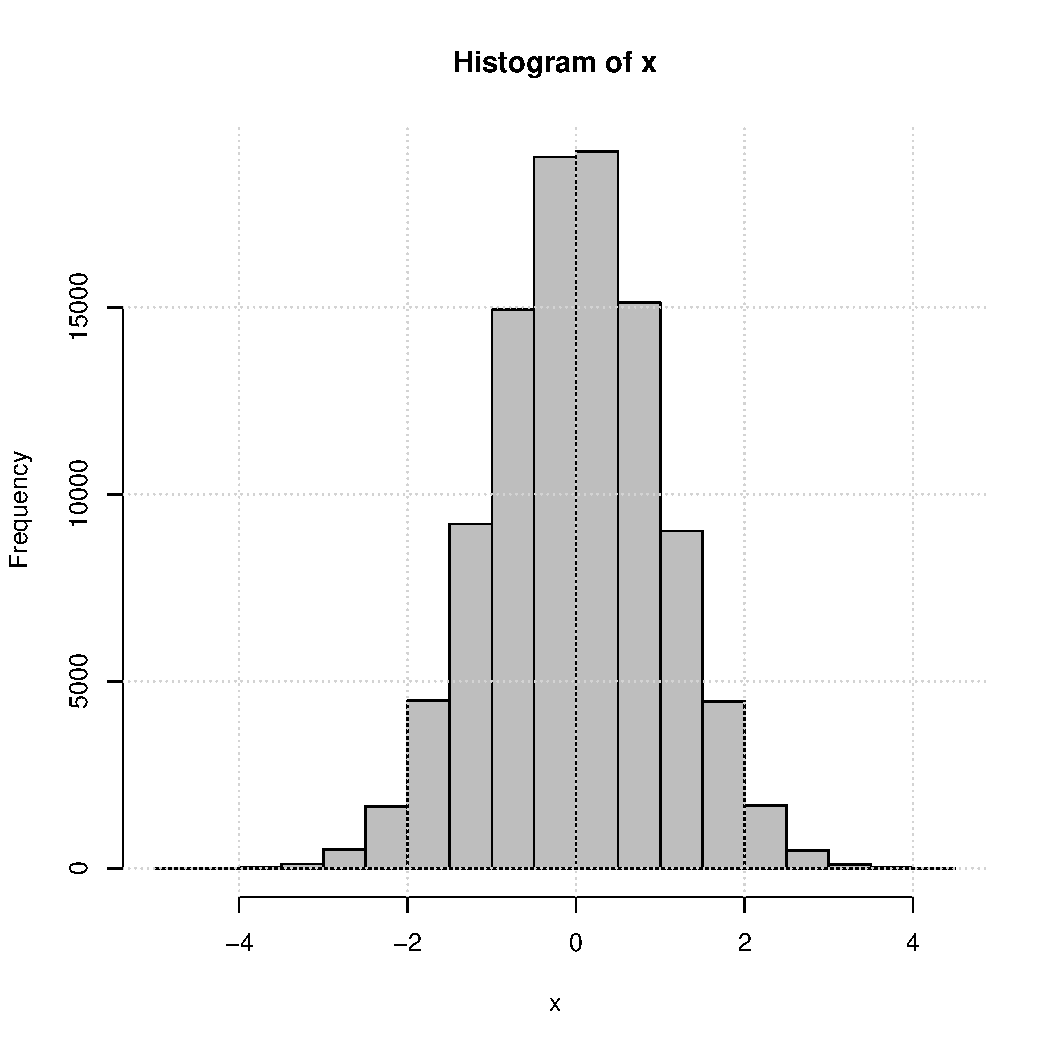
\includegraphics[width=\textwidth]{./figure-1}
  \end{subfigure}

  \captionsetup{margin=10pt,font=small,labelfont=bf,width=.8\textwidth}

  \caption[Krótka nazwa X]{Przykładowy pojedynczy wykres. \textit{Źródło:} opracowanie własne}\label{fig:xxx1}
\end{figure}

\begin{figure}[hbt]
  \centering
  \begin{subfigure}[t]{0.45\textwidth}
    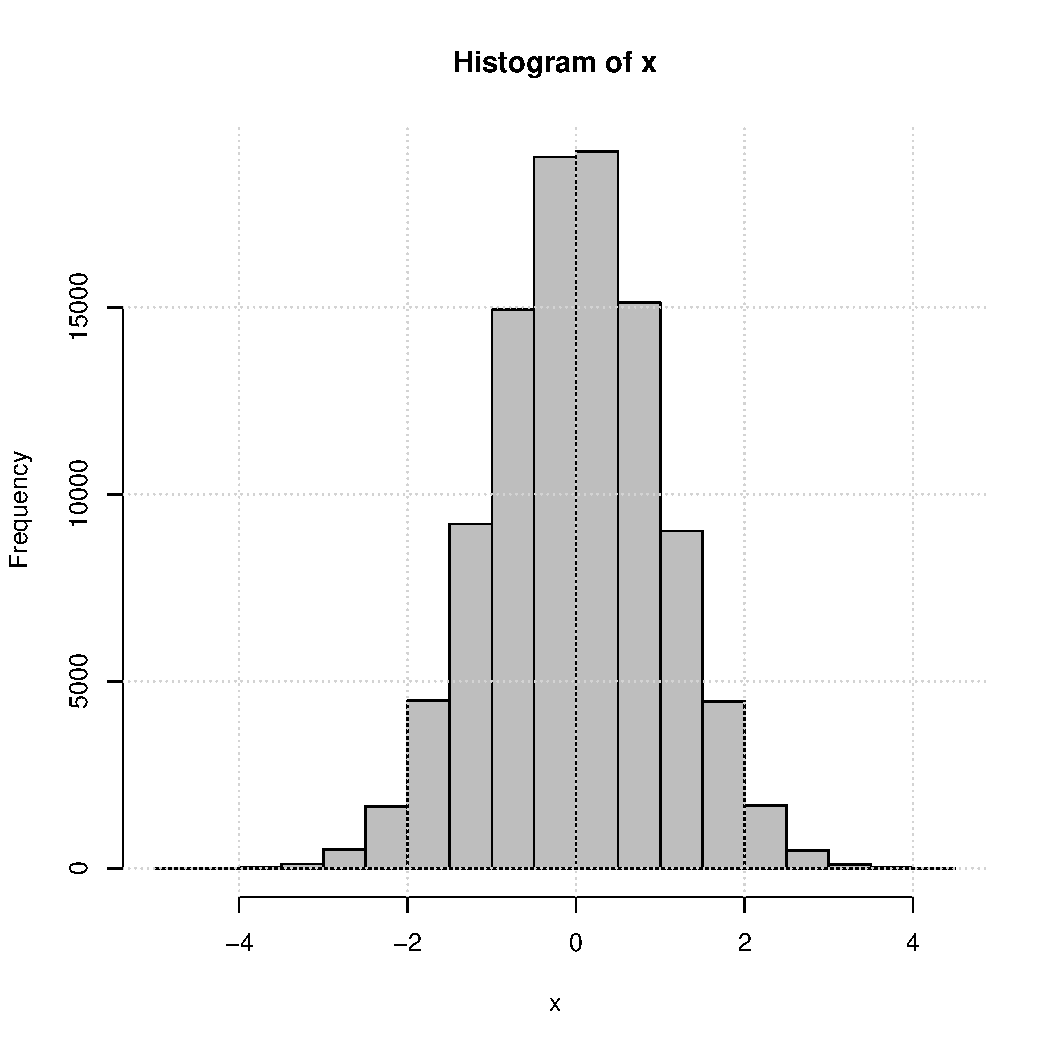
\includegraphics[width=\textwidth]{./figure-1}
    \caption{To jest pierwszy podpis. Ten podpis będzie również zawijany ale będzie to powodowało odpowiednie dopasowanie wysokości.}
    \label{fig:xxxa}
  \end{subfigure}
  \hfill
  \begin{subfigure}[t]{0.45\textwidth}
    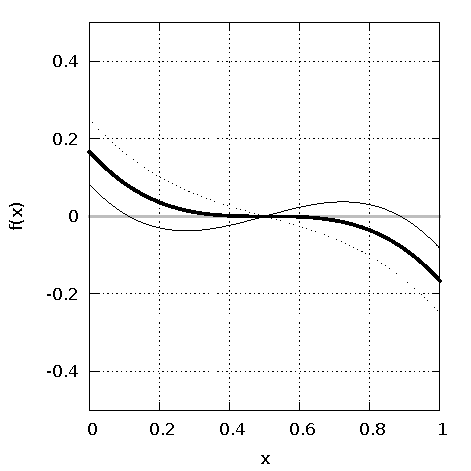
\includegraphics[width=\textwidth]{figure-2}
    \caption{Układ równowag stabilnych}
    \label{fig:xxxb}
  \end{subfigure}
  
  \captionsetup{margin=10pt,font=small,labelfont=bf,width=.8\textwidth}

  \caption[Krótka nazwa II]{Przykładowy wykres. Wykresy podpisujemy, a więc ten opis znajduje się pod wykresem. \textit{Źródło:} opracowanie własne}\label{fig:xxx}
\end{figure}



Odwołanie się do wykresu działa podobnie jak do równania: rysunek~\ref{fig:xxx1}. Możemy również odwoływać się do podwykresów:~\ref{fig:xxxa} lub \ref{fig:xxxb}. Zarówno tablice (tabele) jak i rysunki (wykresy) są automatycznie układane przez \LaTeX{} i nie pozycjinujemy ich sami.

% --- chapter ---------------------------------------------------------
\clearpage
\section{Literatura}

https://www.business.unsw.edu.au/About-Site/Schools-Site/risk-actuarial-site/Documents/A.%20Chernih%20and%20M.%20Sherris%20-%20Spatial%20Risk%20Smoothing.pdf \\




% --- appendices ------------------------------------------------------
\appendix

% ---------------------------------------------------------------------
\clearpage
\section{Dodatek: Ważne rzeczy do dodania}

Tutaj można włożyć długie tablice, kod wykorzystane w pracy lub inne elementy, które nie powinny zakłócać czytania tekstu.


% --- bibliography ----------------------------------------------------
\clearpage
\bibliographystyle{agsm}
\bibliography{refs}

% --- abstract --------------------------------------------------------
\clearpage
\addcontentsline{toc}{section}{Lista tablic}
\listoftables

% --- abstract --------------------------------------------------------
\clearpage
\addcontentsline{toc}{section}{Lista rysunków}
\listoffigures



% --- abstract --------------------------------------------------------
\clearpage
\addcontentsline{toc}{section}{Streszczenie}
\section*{Streszczenie}

Tutaj zamieszczają Państwo streszczenie pracy. Streszczenie powinno być długości około pół strony.


\end{document}

